\scanpage{8}
\mspage{4}
\uline{Ex 1} \unsure{Soient|Soit} \deleted{$k$ un anneau comm.}, $A$ une \deleted{$k$-algèbre} \inserted{ps.-anneau comm.}
$\Omega_A=\mathrm{App}(A,A)$.
Alors en tant que $\mathrm{App}(E,A)$, $A$ ps.ann, $\Omega$ a une structure de ps.ann. comm.
(il est unitaire sss $\deleted{\Omega} A$ est unitaire),
et en tant que $\mathrm{App}(A,A)$, $A$ ens, il a une structure de composition \deleted{\unsure{groupe}} \inserted{monoïdale}, admettant $\mathrm{id}_A$ comme unité.
Les conditions $1^\circ)$ et $2^\circ)$ sont vérifiées.
Les \deleted{applications} éléments ``cts'' de $\Omega$ sont les applications constantes, qui forment un sous-\inserted{ps.}anneau $\Omega_0$ isom. à $A$.
\margin{$\Omega_A$ est unitaire sss $A$ l'est}

\uline{Variante}: si $A$ est une $k$-algèbre \inserted{($k$-ann.comm.unit.)}, on peut prendre
\[
\Omega_{A/k}=\mathrm{End}(W_k(A))
\]
\inserted{(avec $\Omega_0\simeq A$)},
--- plus généralement, si $A$ est un Anneau commutatif sur un topos, on définit
\[
\Omega_{\inserted{A}}\deleted{(\unsure{A})}
=\mathrm{End}_{\substack{\mathrm{faisceaux}\\\mathrm{d'ens.}}}(A),
\]
avec deux structures \deleted{\unsure{d'anneau}} \inserted{$xy$ et $x\circ y$}
(Unitaire si $A$ l'est).
\margin{\figure{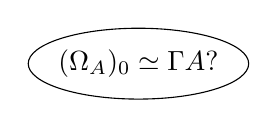
\begin{tikzpicture}\draw (0,0) ellipse (1.4 and .45);\node at (0,0) {$(\Omega_A)_0\simeq\Gamma A$?};\end{tikzpicture}}}

Dans le cas où $A=k$, on trouve $\Omega\simeq k[T]$, où les \inserted{additions,} multiplications et compositions sont celles des polynômes.
Dans ce cas, la condition $3^\circ)$ \unsure{s. les satisf.|satisf. aussi}.
Anneau des constantes est $k$.

On pourra aussi prendre $k[[T]]^+$, avec produit et $x\circ y$,
(l'anneau des ctes est réduit à zero / ou les $a_0+a_1T+\cdots$ avec $a_0$ \uline{nilpotent}
\margin{\unsure{Considérons} \uline{les \unsure{Schémas}} ou ``\uline{\unsure{Anneaux}}'' sur $k$ \uline{\unsure{pro-unip.}}}

\hrule
Soit $\Omega$ un analyseur, $\Omega_0$ le ps.-anneau des ctes, alors
\[
F\longmapsto(\lambda\longmapsto F\circ\lambda):
\Omega\longrightarrow\mathrm{App}(\Omega_0,\Omega_0)=\Omega_{\Omega_0}.
\]
est un ``homo d'analyseurs'', induisant une isom. sur les sous-\inserted{ps.}anneaux des constantes.
On est content quand
\[
\Omega\longrightarrow\deleted{\mathrm{App}}\Omega_{\Omega_0}
\quad\text{est injectif!}
\]
\margin{7}
